\documentclass[letterpaper,11pt]{article}

\usepackage{geometry}
\usepackage{xcolor}
\usepackage{fancyhdr}
\usepackage{graphicx}
\usepackage{parskip}
\usepackage{amsmath,amssymb}
\usepackage{textcomp}
\usepackage{wrapfig}

\title{Earning Our Wages}
\author{SK Gabriel Jagush, Senior Warden\\Worth Commandery \textnumero{} 19, KT}
\date{\textit{Originally published in Volume LXV, Issue \textnumero{} 5,\\of the Knight Templar Magazine, May 2019}}

\begin{document}
	
	\maketitle
	
	The only body of the York Rite that \textit{requires} belief in the Christian faith is the Commandery of Knights
	Templar. However, it is not the only York Rite body that \textit{contains} Christian faith.
	
	We already know that Chivalric Masonry is --– for the most part –-- explicitly Christian. However, the
	Christian faith is seen all over Craft Masonry. While many of the Symbolic, Capitular, and Cryptic degrees
	carry Christian messages (subtle or otherwise), the Mark Master Mason degree in particular teaches a very
	Christian message.
	
	The Mark Master Mason degree is notable among the York Rite Craft degrees for the large volume of
	New Testament verses read throughout, and the fact that the lodge Bible is opened to the Gospel of
	Matthew. However, even if the lodge Bible was opened to a different passage, and there was no reading of
	the New Testament, other characteristics of the degree speak to its powerful Christian message - albeit in a
	more subdued manner.
	
	One notable aspect of the Mark Master Mason degree is the position in which a Mark Master Mason is instructed to place his fingers and hand when receiving his wages. It is a familiar gesture to most modern Christians in the Eastern Orthodox, Byzantine, Oriental, and Nestorian Churches. In both the West and East, when Christians make the Sign of the Cross, they touch their forehead, chest, and shoulders with their right hand. There are variances in order of movements, how far down on the chest one makes contact, and so forth, but the most notable difference between the two methods is the position of the hand and fingers. 
	
	\pagebreak
	
	\begin{wrapfigure}{r}{0.45\textwidth}
		\begin{center}
			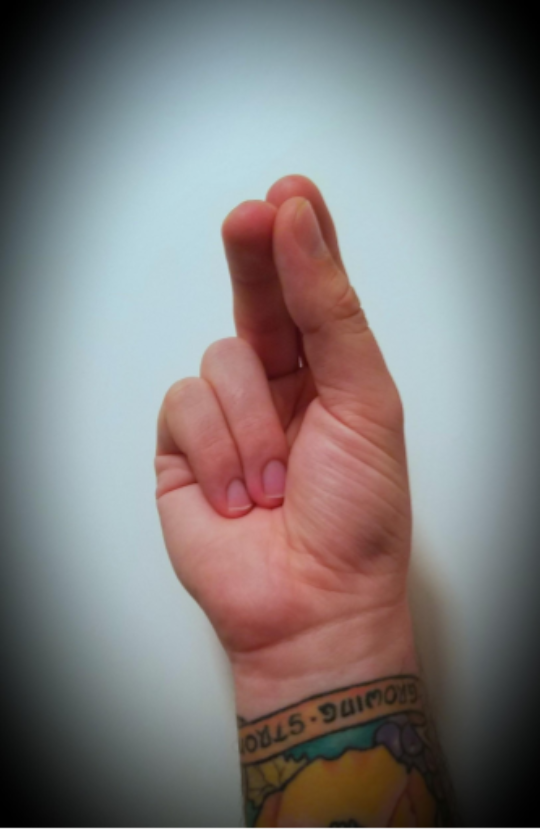
\includegraphics[width=0.4\textwidth]{MarkMasterHand.png}
			\caption{\small{Position of fingers while making the \textit{Sign of the Cross} in the Byzantine fashion, as demonstrated by author.}}
		\end{center}
	\end{wrapfigure}
	
	To speak in broad strokes, many Western Christians tend to use an open hand with all five fingers to symbolize the Five Wounds of Christ, or the index, middle, and ring fingers placed together, but many Eastern Christians place their thumb, index, and middle fingers together, with the little and ring finger tucked into the palm. The three fingers held together are a reminder that the Father, Son, and Holy Ghost are three distinct Persons who are of one Substance in the Godhead. The two fingers tucked into the palm are a reminder of the hypostatic union of Christ as the fully human Jesus of Nazarene and the fully Divine Son of God.
	
	What, then, does this particular hand positioning mean for us as Knights Templar, and how might it relate to the Mark Master Mason degree?
	
	This same positioning used to make the Sign of the Cross is also the same positioning used to receive our wages as Mark Master Masons. By holding our Mark against our palms with our little and ring fingers, we are enabled to receive our wages between our thumb, index, and middle fingers. Those without a Mark cannot receive their wages. In the same way, by placing our faith in Christ who was simultaneously Man and God, we are enabled to receive eternal salvation through the Divine grace of the Godhead. Without grace, we cannot enter heaven.
	
	As Knights Templar, we are also, by definition, Mark Master Masons. We know that there is more to the story than earning a penny after a day's work. Our Mark is our faith in Christ, and our wage is salvation.
	
\end{document}